\documentclass[../main.tex]{subfiles}

\begin{document}

\section{Exercise 2.1}

Code:

\begin{lstlisting}
(define (make-rat n d)
  (if (< d 0)
      (make-rat (- 0 n) (- 0 d))
      (let ((g (gcd n d)))
        (cons (/ n g) (/ d g)))))
\end{lstlisting}

\section{Exercise 2.2}

Code:

\begin{lstlisting}
;; point definition
(define (make-point x y)
  (cons x y))
(define (x-point point)
  (car point))
(define (y-point point)
  (cdr point))

;; segment definition
(define (make-segment start end)
  (cons start end))
(define (start-segment segment)
  (car segment))
(define (end-segment segment)
  (cdr segment))
(define (midpoint-segment segment)
  (define (average x y)
    (/ (+ x y) 2.0))
  (let ((start (start-segment segment))
        (end (end-segment segment)))
    (make-point (average (x-point start)
                         (x-point end))
                (average (y-point start)
                         (y-point end)))))
\end{lstlisting}

\section{Exercise 2.3}

Code:

\begin{lstlisting}
;; one version of rectangle
(define (make-rect top-left bottom-right)
  (cons top-left bottom-right))
(define (top-left rect)
  (car rect))
(define (bottom-right rect)
  (cdr rect))
(define (width rect)
  (- (x-point (bottom-right rect))
     (x-point (top-left rect))))
(define (height rect)
  (- (y-point (bottom-right rect))
     (y-point (top-left rect))))

;; another version of rectangle
(define (make-rect top-left width height)
  (cons top-left (cons width height)))
(define (top-left rect)
  (car rect))
(define (width rect)
  (car (cdr rect)))
(define (height rect)
  (cdr (cdr rect)))

;; rect procedures
(define (perimeter rect)
  (* 2 (+ (width rect) (height rect))))
(define (area rect)
  (* (width rect) (height rect)))
\end{lstlisting}

\section{Exercise 2.4}

By evaluating \lstinline{(car (cons x y))} using
 applicative-order strategy, it can be verified
 that \lstinline{(car (cons x y))} yields
 \lstinline{x} for any object \lstinline{x} and
 \lstinline{y}:

\begin{lstlisting}
(car (cons x y)) ->
(car (lambda (m) (m x y))) ->
((lambda (m) (m x y)) (lambda (p q) p)) ->
((lambda (p q) p) x y) ->
x
\end{lstlisting}

The same result can also be obtained using
 normal-order strategy:

\begin{lstlisting}
(car (cons x y)) ->
((cons x y) (lambda (p q) p)) ->
((lambda (m) (m x y)) (lambda (p q) p)) ->
((lambda (p q) p) x y) ->
x
\end{lstlisting}

The corresponding definition of \lstinline{cdr}:

\begin{lstlisting}
(define (cdr z)
  (z (lambda (p q) q)))
\end{lstlisting}

\section{Exercise 2.5}

Code:

\begin{lstlisting}
(define (cons x y)
  (* (expt 2 x) (expt 3 y)))
(define (car z)
  (define (car-iter z sum)
    (if (= (remainder z 2) 0)
        (car-iter (/ z 2) (+ 1 sum))
        sum))
  (car-iter z 0))
(define (cdr z)
  (define (cdr-iter z sum)
    (if (= (remainder z 3) 0)
        (cdr-iter (/ z 3) (+ 1 sum))
        sum))
  (cdr-iter z 0))
\end{lstlisting}

\section{Exercise 2.6}

Code:

\begin{lstlisting}
(define one (lambda (f) (lambda (x) (f x))))
(define two (lambda (f) (lambda (x) (f (f x)))))
(define (add a b)
  (lambda (f) (lambda (x) ((a f) ((b f) x)))))
\end{lstlisting}

\section{Exercise 2.7}

Code:

\begin{lstlisting}
(define (upper-bound interval)
  (car interval))
(define (lower-bound interval)
  (cdr interval))
\end{lstlisting}

\section{Exercise 2.8}

The difference of two intervals is the
 sum of the first and the opposite interval
 of the second.

Code:

\begin{lstlisting}
(define (sub-interval x y)
  (define (neg-interval x)
    (make-interval (- 0 (upper-bound x)) (- 0 (lower-bound x))))
  (add-interval x (sub-interval y)))
\end{lstlisting}

\section{Exercise 2.9}

Let $(a, b)$ denote an interval with
 lower bound $a$ and upper bound $b$.

For any two intervals $p=(p_l, p_u)$
 and $q=(q_l, q_u)$ with widths $W_p = \frac{p_u - p_l}{2}$
 and $W_q = \frac{q_u - q_l}{2}$
 respectively, the sum of $p$ and $q$ is
 $(p_l + q_l, p_u + q_u)$, whose width is
 $\frac{(p_u + q_u) - (p_l + q_l)}{2} =
 \frac{(p_u - p_l) + (q_u - q_l)}{2} = W_p + W_q$.

Similarly, the difference of $p$ and $q$ is
 $(p_l - q_u, p_u - q_l)$, whose width is
 $\frac{(p_u - q_l) - (p_l - q_u)}{2} = 
 \frac{(p_u - p_l) + (q_u - p_l)}{2} = W_p + W_q$.

Therefore, the width of the sum (or difference) of two
 intervals is a function only of the widths of the intervals
 being added (or subtracted).

Two examples illustrating that this is not true for
 multiplication or division are as follows:

\begin{itemize}
\item The width of $(0, 1) * (1, 2) = (1, 2)$ is $\frac{1}{2}$,
 while the width of $(1, 2) * (1, 2) = (1, 4)$ is $\frac{3}{2}$.
\item The width of $\frac{(0, 1)}{(1, 2)} = (0, 1) *
 (\frac{1}{2}, 1) = (0, \frac{1}{2})$ is $\frac{1}{4}$,
 while the width of $\frac{(1, 2)}{(1, 2)} = (1, 2) *
 (\frac{1}{2}, 1) = (\frac{1}{2}, 2)$ is $\frac{3}{4}$.
\end{itemize}

\section{Exercise 2.10}

Code:

\begin{lstlisting}
(define (div-interval x y)
  (define (exclude-zero? interval)
    (or (< (upper-bound interval) 0)
        (> (lower-bound interval) 0)))
  (if (exclude-zero? y)
    (mul-interval x
                  (make-interval (/ 1.0 (upper-bound y))
                                 (/ 1.0 (lower-bound y))))))
\end{lstlisting}

\section{Exercise 2.11}

Code:

\begin{lstlisting}
(define (mul-interval x y)
  (let ((x0 (lower-bound x))
        (x1 (upper-bound x))
        (y0 (lower-bound x))
        (y1 (upper-bound y)))
    (if (> x0 0)
        (if (> x1 0)
            (if (> y0 0)
                (if (> y1 0)
                    (make-interval (* x0 y0) (* x1 y1)))
                (if (> y1 0)
                    (make-interval (* x1 y0) (* x1 y1))
                    (make-interval (* x1 y1) (* x0 y0)))))
      (if (> x1 0)
          (if (> y0 0)
              (if (> y1 0)
                  (make-interval (* x0 y1) (* x1 y1)))
              (if (> y1 0)
                  (make-interval (min (* x0 y1) (* x1 y0)) (* x1 y1))
                  (make-interval (* x1 y1) (* x0 y1))))
          (if (> y0 0)
              (if (> y1 0)
                  (make-interval (* x0 y1) (* x1 y0)))
              (if (> y1 0)
                  (make-interval (* x0 y1) (* x1 y0))
                  (make-interval (* x1 y0) (* x0 y1)))))))
\end{lstlisting}

\section{Exercise 2.12}

Code:

\begin{lstlisting}
(define (make-center-percent center percent)
  (make-center-width center (* percent center)))
(define (percent interval)
  (/ (width interval) (center interval)))
\end{lstlisting}

\section{Exercise 2.13}

Let $x$ be an interval with average $a_0$ and tolerance $t_0$,
 $y$ be an interval with average $a_1$ and tolerance $t_1$, then we have:

\begin{align*}
x &= (a_0 - a_0 t_0, a_0 + a_0 t_0) \\
y &= (a_1 - a_1 t_1, a_1 + a_1 t_1)
\end{align*}

Assume that all numbers are positive (no non-positive numbers
 are included in any of the intervals), then we have:

\begin{align*}
x \cdot y &= ((a_0 - a_0 t_0)(a_1 - a_1 t_1), (a_0 + a_0 t_0)(a_1 + a_1 t_1)) \\
&= (a_0 a_1 - a_0 a_1 (t_0 + t_1) + a_0 a_1 t_0 t_1, a_0 a_1 + a_0 a_1 (t_0 + t_1) + a_0 a_1 t_0 t_1)
\end{align*}

Denote $x \cdot y$ as $(u, v)$, then the tolerance of $x \cdot y$ is:

\begin{align*}
\frac{\frac{v-u}{2}}{\frac{v+u}{2}} &= \frac{a_0 a_1 (t_0 + t_1)}{a_0 a_1 + a_0 a_1 t_0 t_1} \\
&= \frac{t_0 + t_1}{1 + t_0 t_1}
\end{align*}

\section{Exercise 2.14}

For $R_1 = (1, 2)$ and $R_2 = (2, 3)$, $\frac{R_1 R_2}{R_1 + R_2} = (\frac{2}{5}, 2)$, while
$\frac{1}{1/R_1 + 1/R_2} = (\frac{2}{3}, \frac{5}{6})$

\section{Exercise 2.15}

\lstinline{par2} is indeed better, but for a different reason.

In $\frac{R_1 R_2}{R_1 + R_2}$, we want to refer to the same variable
 when referring to $R_1$ in numerator and demonimator. However, we are
 actually treating them as if they're independent of each other. Using
 \lstinline{par2} there won't be such issue.

\section{Exercise 2.16}

Because the operands are random variables instead of real values. This
 could bring severe problems. For example, when we write $\frac{(1, 2)}{(1, 2)}$,
 there's no way to tell if we are referring to an interval divided by itself,
 or an interval divided by another with the same distribution. For the former
 result should be 1 (or written as $(1, 1)$ in interval format), for the latter
 result should be $(\frac{1}{2}, 2)$. This kind of ambiguity determines that
 it's impossible to devise such arithmetic package for intervals.

\section{Exercise 2.17}

Code:

\begin{lstlisting}
(define (last-pair lst)
  (if (null? (cdr lst))
      lst
      (last-pair (cdr lst))))
\end{lstlisting}

\section{Exercise 2.18}

Code:

\begin{lstlisting}
(define (reverse lst)
  (define (reverse-iter new lst)
    (if (null? lst)
        new
        (reverse-iter (cons (car lst) new) (cdr lst))))
  (reverse-iter (list) lst))
\end{lstlisting}

\section{Exercise 2.19}

Code:

\begin{lstlisting}
(define (first-denomination coin-values)
  (car coin-values))
(define (except-first-denomination coin-values)
  (cdr coin-values))
(define (no-more? coin-values)
  (null? coin-values))
\end{lstlisting}

The order of the list \lstinline{coin-values} does not
 affect the answer produced. Given an amount and a
 list of coin values, whatever the order is, there are
 only two cases, which are to use the first type of coin
 in the list or not. Therefore, the procedure \lstinline{cc}
 performs a complete search in solution space, which
 is not dependent of the order of \lstinline{coin-values}.

\section{Exercise 2.20}

Code:

\begin{lstlisting}
(define (same-parity i . lst)
  (let ((parity (remainder i 2)))
    (define (same? x)
      (= (remainder x 2) parity))
    (define (filter lst)
      (if (null? lst)
          (list)
          (if (same? (car lst))
              (cons (car lst) (filter (cdr lst)))
              (filter (cdr lst)))))
    (cons i (filter lst))))
\end{lstlisting}

\section{Exercise 2.21}

Code:

\begin{lstlisting}
(define (square-list items)
  (define (square x) (* x x))
  (if (null? items)
      items
      (cons (square (car items)) (square-list (cdr items)))))
(define (square-list items)
  (map (lambda (x) (* x x))
       items)
\end{lstlisting}

\section{Exercise 2.22}

In the first version, the procedure inserts
 each result to the head of the answer list
 while iterating over the original list, thus
 the answer list is in reverse order.

In the second version, applying \lstinline{cons}
 to a list and a number produces a new list with
 the given list be the first element and the given
 number be the second element instead of the result
 of appending the given number to the given list.

\section{Exercise 2.23}

Code:

\begin{lstlisting}
(define (for-each fn lst)
  (if (null? lst)
      lst
      ((lambda (lst) (fn (car lst)) (for-each fn (cdr lst))) lst)))
\end{lstlisting}

\section{Exercise 2.24}

Interpreter output:

\begin{lstlisting}
(1 (2 (3 4)))
\end{lstlisting}

Box-n-pointer structure:

\begin{lstlisting}
* -> */
|    |
1    * -> */
     |    |
     2    * -> */
          |    |
          3    4
\end{lstlisting}

Tree interpretation:

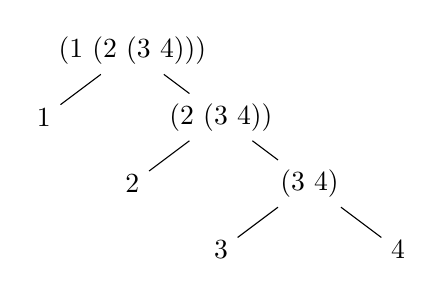
\begin{tikzpicture}[sibling distance=64pt, level distance=24pt]
\node{\lstinline{(1 (2 (3 4)))}}
  child{node{\lstinline{1}}}
  child{node{\lstinline{(2 (3 4))}}
    child{node{\lstinline{2}}}
    child{node{\lstinline{(3 4)}}
      child{node{\lstinline{3}}}
      child{node{\lstinline{4}}}}};
\end{tikzpicture}

\section{Exercise 2.25}

Code:

\begin{lstlisting}
(let ((l (list 1 3 (list 5 7) 9)))
  (car (cdr (car (cdr (cdr l))))))
(let ((l (list (list 7))))
  (car (car l)))
(let ((l (list 1 (list 2 (list 3 (list 4
  (list 5 (list 6 7))))))))
  (car (cdr (car (cdr (car (cdr (car (cdr
    (car (cdr (car (cdr l)))))))))))))
\end{lstlisting}

\section{Exercise 2.26}

The results are respectively
\lstinline{(1 2 3 4 5 6)},
\lstinline{((1 2 3) 4 5 6)},
and \lstinline{((1 2 3) (4 5 6))}.

\section{Exercise 2.27}

Code:

\begin{lstlisting}
(define (deep-reverse lst)
  (define (reverse-iter new lst)
    (define (reverse-elem elem)
      (if (list? elem)
          (reverse-iter (list) elem)
          elem))
    (if (null? lst)
        new
        (reverse-iter (cons (reverse-elem (car lst)) new) (cdr lst))))
  (reverse-iter (list) lst))
\end{lstlisting}

\section{Exercise 2.28}

Code:

\begin{lstlisting}
(define (fringe t)
  (if (list? t)
      (if (null? t)
          t
          (append (fringe (car t))
                  (fringe (cdr t))))
      (list t)))
\end{lstlisting}

\section{Exercise 2.29}

\subsection{a.}

Code:

\begin{lstlisting}
(define (left-branch mobile)
  (car mobile))
(define (right-branch mobile)
  (car (cdr mobile)))
(define (branch-length branch)
  (car branch))
(define (branch-structure branch)
  (car (cdr branch)))
\end{lstlisting}

\subsection{b.}

Code:

\begin{lstlisting}
(define (total-weight mobile)
  (+ (branch-weight (left-branch mobile))
     (branch-weight (right-branch mobile))))
\end{lstlisting}

\subsection{c.}

Methods to be rewritten:

\begin{lstlisting}
(define (right-branch mobile)
  (cdr mobile))
(define (branch-structure branch)
  (cdr branch))
\end{lstlisting}

\section{Exercise 2.30}

Code defining \lstinline{square-tree} directly:

\begin{lstlisting}
(define (square-tree t)
  (cond ((null? t) t)
        ((not (pair? t)) (* t t))
        (else (cons (square-tree (car t))
                    (square-tree (cdr t))))))
\end{lstlisting}

Code defining the same method using higher-order
 procedures:
 
\begin{lstlisting}
(define (square-tree t)
  (map (lambda (subtree)
         (if (pair? subtree)
           (square-tree subtree)
           (* subtree subtree)))
       t))
\end{lstlisting}

\section{Exercise 2.31}

Code:

\begin{lstlisting}
(define (tree-map method t)
  (map (lambda (subtree)
         (if (pair? subtree)
           (tree-map method subtree)
           (method subtree)))
       t))
\end{lstlisting}

\section{Exercise 2.32}

Code:

\begin{lstlisting}
(define (subsets s)
  (if (null? s)
      (list '())
      (let ((rest (subsets (cdr s))))
        (append rest (map (lambda (x)
                            (cons (car s) x))
                          rest)))))
\end{lstlisting}

\section{Exercise 2.33}

Code:

\begin{lstlisting}
(define (accumulate op initial seq)
  (if (null? seq)
      initial
      (op (car seq)
          (accumulate op initial (cdr seq)))))
(define (map p sequence)
  (accumulate (lambda (x y) (cons (p x) y)) (list) sequence))
(define (append seq1 seq2)
  (accumulate cons seq2 seq1))
(define (length sequence)
  (accumulate (lambda (x y) (+ 1 y)) 0 sequence))
\end{lstlisting}

\section{Exercise 2.34}

Code:

\begin{lstlisting}
(define (horner-eval x coefficient-sequence)
  (accumulate (lambda (this-coeff higher-terms)
                (+ this-coeff (* x higher-terms)))
              0
              coefficient-sequence))
\end{lstlisting}

\section{Exercise 2.35}

Code:

\begin{lstlisting}
(define (count-leaves t)
  (accumulate +
              0
              (map (lambda (subtree)
                     (if (not (pair? subtree))
                         1
                         (+ (count-leaves (car subtree))
                            (count-leaves (cdr subtree)))))
                   t)))
\end{lstlisting}

\end{document}










